\begin{example} \label{eg:6.4.2} % EXAMPLE
A thin bar occupies the interval $0 \leq x \leq 2$ and it has a density in kg/m of $\rho(x) = 1+ x^2$. Find the center of mass of the bar. 

\solution
From Example \ref{eg:6.4.1}, the mass of the bar in kilograms is $\frac{14}{3}$ kg. We just need to find $\int_a^b x \rho(x) \ dx$.
\begin{align*}
	\int_a^b \rho(x) \ dx  & = 	\int_0^2 x (1+x^2) \ dx \\
		&= \int_0^2 (x +x^3) \ dx \\
		&= 	\left(\frac{x^2}{2}+\frac{x^4}{4} \right) \Big|_0^2 \\
		&= 8.
\end{align*}
The center of mass, $\overline{x}$, 00is $\frac{8}{14/3} = \frac{12}{7}$. 

\end{example}

%\begin{marginfigure}[-8cm] %MARGIN FIGURE
%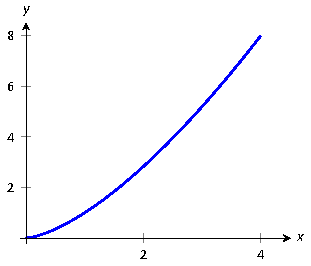
\includegraphics{figures/figarc1}
%\caption{A graph of $f(x) = x^{3/2}$ from Example~\ref{eg:6.3.1}.} \label{F:6.3.Ex1}
%\end{marginfigure}

